% !TEX program = pdflatex
% !TEX options = -synctex=1 -interaction=nonstopmode -file-line-error -shell-escape "%DOC%"
\documentclass{beamer}
\usepackage{graphicx,url}
\usepackage[brazil]{babel}   
\usepackage[utf8]{inputenc}
\usepackage{pgf,tikz}
\usepackage{adjustbox}
\usepackage{mathrsfs}
\usepackage{minted}
\usepackage{listings}
\usetikzlibrary{calc}
\usetikzlibrary{arrows}
\batchmode
\usepackage{amsmath,amssymb,enumerate,epsfig,bbm,calc,color,ifthen,capt-of}
\usetheme{Berlin}
%-------------------------Titulo/Autores/Orientador------------------------------------------------
\title[Introduction to Competitive Programming]{
Introduction to Competitive Programming
}
\subtitle {MCPC-2020 Winter Training}
\date{}
\author[Shizhe Zhao (eggeek)]{
  Shizhe Zhao (eggeek)
}

\pgfdeclareimage[height=0.7cm]{monash-logo}{icpc.pdf}
\logo{\pgfuseimage{monash-logo}\hspace*{0.5cm}}

% \AtBeginSection[]
% {
%   \begin{frame}<beamer>
%     \frametitle{Outline}
%     \tableofcontents[currentsection]
%   \end{frame}
% }
% \setbeamercovered{transparent}
% \beamerdefaultoverlayspecification{<+->}
% -----------------------------------------------------------------------------
\begin{document}
% -----------------------------------------------------------------------------

%---Summary---------------------------------------------------------
\frame{\titlepage}
\section[]{}
% \begin{frame}{Summary}
%   \tableofcontents
% \end{frame}

\section{Overview}
\begin{frame}{About the training}
  \begin{itemize}
    \item There will be 2 - 3 workshops in winter
    \item To cover: problem solving, C++ and data structures
    \item Training contests will be on: \url{https://vjudge.net/group/monashicpc}
  \end{itemize}
  Note that, this training \textbf{is not}:
  \begin{itemize}
    \item for your coursework
    \item for tech-interview and software development
    \item although it helps things above, a lot.
  \end{itemize}
  It \textbf{is}
  \begin{itemize}
    \item developing your problem-solving skill
    \item filling up the gap between your coursework and practice
  \end{itemize}
\end{frame}

\section{Problem Solving}
\begin{frame}{Basic Strategy: Brute-force}
  \begin{itemize}
    \item Helps you understand the problem
    \item Good start-point before implementing a complicate algorithm
    \item Examples ...
  \end{itemize}
\end{frame}

\begin{frame}
  \frametitle{Brute-force example: anticolockwise motion \textit{\small(SP-ICPC 2016)}}
\begin{minipage}{.4\textwidth}
\begin{figure}[]
  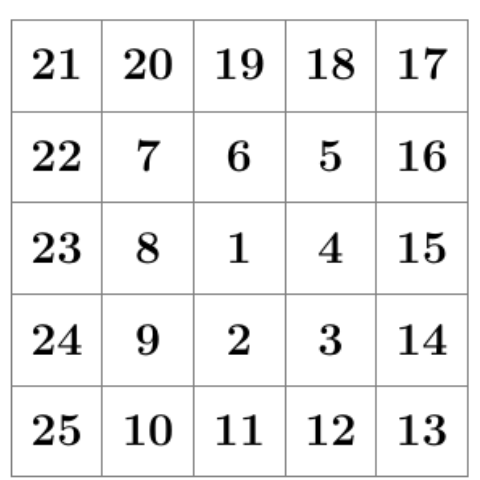
\includegraphics[width=1.0\textwidth]{pics/anticolockwise.png} 
\end{figure} 
\end{minipage}%
\begin{minipage}{.6\textwidth}
  \only<1>{
    Q: What's the location of $n \leq 10^{10}$ ?
  }
  \only<2-3>{

    Brute-force thinking ($O(n)$):

    simulate the "motion" for $n$ steps.
    \vspace{3mm}
  }
  \only<3->{


    Popping up sub-questions:
    \begin{itemize}
      \item start-up direction?
      \item \#num of steps?
      \item when direction change?
    \end{itemize}
  }
  \only<4-> {

    Wait, since you know \textbf{\#num of steps},
    you don't need to simulate each motion ...

    \onslide<5-> {

      Which will be $O(\sqrt{n})$!
    }
  }

\end{minipage}
\end{frame}

\begin{frame}
  \frametitle{Brute-force example: runtime analysis}

\textbf{Keep in mind:}

You can assume, C++ simulates $10^8$ (Python: $10^6$) "steps" (i.e. CPU operations) per second,

\vspace{3mm}
Thus, the estimated time of an $O(n)$ solution is $\mathbf{100s}$ when $n=10^{10}$, 
while an $O(\sqrt{n})$ solution is $\mathbf{0.001s}$; there are orders of magnitude difference!

\end{frame}

\begin{frame}
  \frametitle{Brute-force example: further thinking}
\begin{itemize}
  \item Can we do this better than $O(\sqrt{n})$?
  \item What if the moving-pattern is in rectangle instead of square?
  \item What if cells are: \textit{triangles}, \textit{hexagons}?
\end{itemize}  

\end{frame}

\begin{frame}
  \frametitle{Anti Brute-force example: Fast and Furious$^*$ \textit{\small(MCPC 2020)}}
\begin{minipage}{.3\textwidth}
  \hspace{-8mm}
  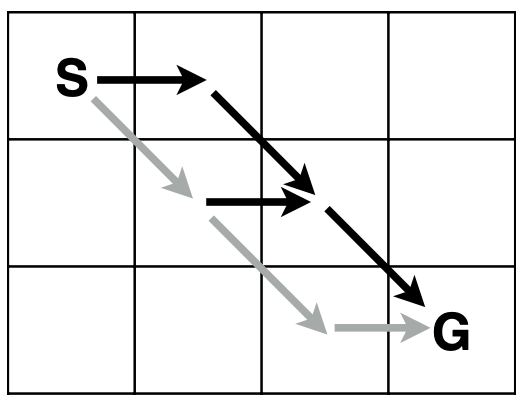
\includegraphics[width=1.1\textwidth]{pics/grid.png} 
\end{minipage}%
\begin{minipage}{.7\textwidth}
  \begin{itemize}
    \item\onslide<1->{
      Q: In infinite grid-map, given $\mathbf{m}$, 
      find a path that minimize the steps from \textbf{S} to \textbf{G}, 
      while direction must be different at second $\mathbf{k*m}$ and $\mathbf{k*m+1}$, for any $k>0$.
    }
    \item\onslide<2->{

      Brute-force thinking:

      Move on the shortest path (\textit{on which?}), change direction (\textit{to which?}) when necessary (\textit{when?}).
    }
    \item\onslide<3-> {
      You will able to write a program now.

      But wait, \textbf{how to guarantee correctness?}
    }
  \end{itemize}
\end{minipage}
\end{frame}

\begin{frame}
  \frametitle{Anti Brute-force example: Fast and Furious$^*$ \textit{\small(MCPC 2020)}}
\begin{minipage}{.3\textwidth}
  \hspace{-8mm}
  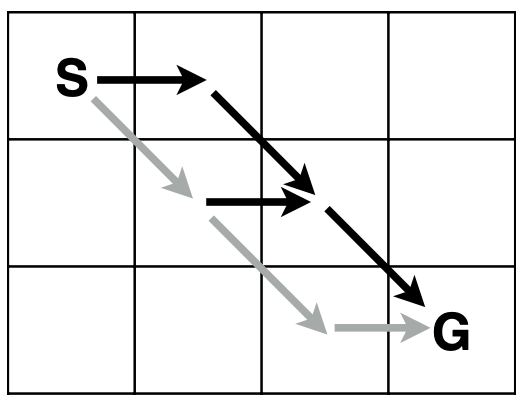
\includegraphics[width=1.1\textwidth]{pics/grid.png} 
\end{minipage}%
\begin{minipage}{.7\textwidth}
  \begin{itemize}
    \item<1-> {
      Approach 1 (brute-force):


      This problem is actually in 3D space - \textit{(x, y, time)};
      and your brute-force simulation should based on this.


      (conceptually easier, practically harder)
    }

    \item<2-> {
      Approach 2 (greedy):

      Minimize $|dx - dy|$ in each step.


      (conceptually harder, practically easier)
    }
    
    \item<3-> {
      And many other approaches ...
    }

  \end{itemize}
\end{minipage}
\end{frame}

\section{Programming}
\begin{frame}
  \frametitle{Use c/c++!}

Annoying things in c++:

\begin{itemize}
  \item {
    pointers
    \onslide<2-> {
      $\rightarrow$ you \textbf{don't need} to use pointers in contest
    }
  }
  \item {
    memory leaking
    \onslide<2-> {
      $\rightarrow$ you \textbf{don't need} dynamic memory allocation in contest
    }
  }
  \item {
    complicated paradigm
    \onslide<2-> {
      $\rightarrow$ you \textbf{only} need simple paradigm in contest
    }
  }
  \item {
    building system
    \onslide<2-> {
      $\rightarrow$ you \textbf{only} need to compile single file in contest
    }
  }
  \item {
    using third-party packages
    \onslide<2-> {
      $\rightarrow$ you can \textbf{only} use builtin libraries in contest
    }
  }
\end{itemize}
  
\onslide<3-> {
  Rest parts of c/c++ are sweet!
}
\end{frame}

\begin{frame}[fragile]
  \frametitle{Sweet c/c++: compile single file}
TL;DR:
\begin{minted}[linenos=false, frame=lines, fontsize=\footnotesize]{sh}
  # minimum, get executable a.out
  g++ myalgo.cc
  # specify optimize level for debugging
  g++ myalgo.cc -g -O0 -Wall -o myalgo
  # specify optimize level for running
  g++ myalgo.cc -O3 -o myalgo
\end{minted}
\begin{itemize}
  \item compiler: e.g. \texttt{gcc, g++, clang, clang++}
  \item path of source file: e.g. \texttt{myalgo.\{c,cc,cpp\}}
  \item argvs
    \begin{itemize}
      \item \texttt{-g [-O0]}: for debugging, slow but more conservative
      \item \texttt{-O[0/1/2/3]}: for running, fast and well optimized
      \item \texttt{-o}: set executable name, default is \texttt{a.out}
    \end{itemize}
\end{itemize}

\end{frame}

\begin{frame}[fragile]
  \frametitle{Sweet c/c++: no malloc}
\begin{minted}[linenos=true, frame=lines, fontsize=\footnotesize]{c++}
// N is the upper bound given by problem statement
const int N = 100;

// use static memory and int index
int arr[N], cnt;

cnt = 0;                  // "clean" memory
for (int i=0; i<m; i++) {
  arr[cnt++] = dummyelem  // add element
}
\end{minted}
\end{frame}

\begin{frame}[fragile]
  \frametitle{Sweet c/c++: no pointers}
\begin{minted}[linenos=true, frame=lines, fontsize=\footnotesize]{c++}
// stack  
int stack[N], cnts = 0;     // clear
stack[cnts++] = dummy_elem; // push stack
dummy_elem = stack[--cnts]; // pop  stack

// queue
int que[N], front, tail;
front = tail = 0;           // clear
que[tail++] = dummy_elem;   // push queue
dummy_elem = que[front++];  // pop queue

// circular queue
tail  = (tail + 1) % size   // when push
front = (front + 1) % size  // when pop
\end{minted}
\end{frame}

\begin{frame}[fragile]
  \frametitle{Sweet c/c++: no pointers}
\begin{minted}[linenos=true, frame=lines, fontsize=\footnotesize]{c++}
// sort
int arr[N], n = 10;

// sort arr[0:n-1]
sort(arr, arr+n);

// sort with specified compare function
bool cmp(int x, int y) { return x < y; }
sort(arr, arr+n, cmp);
\end{minted}
\end{frame}


\begin{frame}[fragile]
  \frametitle{Sweet c/c++: looping}

\textbf{\textcolor{red}{Very important}:}
\begin{itemize}
  \item \textbf{Pre-condition:} what should be true before the loop;
  \item \textbf{Invariant:} what should be maintained by the loop;
  \item \textbf{Post-condition:} what should be true after the loop;
\end{itemize}
Most of bugs are caused by mistakes on them.
\begin{example}
  \footnotesize{
  In the problem \textbf{Fast ad Furious}, you decide to simulate the motion 
  based on the brute-force thinking (on shortest path and change direction when necessary).
  But note that changing direction may cause the agent away from the shortest path, and thus break
  your \textbf{invariant}.
  }
\end{example}

Try to apply these concepts to explain why pointer-free stack, queue and circular queue work (previous page).
\end{frame}

\begin{frame}[fragile]
  \frametitle{Sweet c/c++: looping}
\begin{minted}[linenos=true, frame=lines, fontsize=\footnotesize]{c++}
// for-loop
for (<pre-cond>; <invariant>; <action>) { <actions> }
// example:
for (int i=0; i<n; i++) {
  que[tail++] = dummy_elem;
}
// another example:
int i = 0;
for ( ; ; ) {
  if (i >= n) break;
  que[tail++] = dummy_elem;
  i++;
}
\end{minted}
There are also \textbf{while-loop} and \textbf{do-while} in c/c++, 
but they are interchangeable with \textbf{for-loop}.

\end{frame}

\begin{frame}[fragile]
  \frametitle{Sweet c/c++: standard IO}
C/C++ input is stream-based which will tokenize the content, while Python is line-based.

Example:

For input text \texttt{"Year 2020\textbackslash n"}, c/c++ regard it as\\
 \texttt{["Year", "2020"]};
while Python will read the whole line, and further parsing is required.

\begin{minted}[linenos=false, frame=lines, fontsize=\footnotesize]{c++}
// stream-based input
char str[N]; int year;
scanf("%s %d", str, &year);
// get whole line
char line[N];
gets(line); // this is unsafe in practice, but fine in contest
\end{minted}

\end{frame}

\begin{frame}
  \frametitle{Resources}
\begin{itemize}
  \item C/C++ IO - \url{https://vjudge.net/contest/361790}
  \item Training contest - \url{https://vjudge.net/contest/383886}
  \item Extra resources for problem solving: 
  \begin{itemize}
    \item GCJ Round-1 \url{https://codingcompetitions.withgoogle.com/codejam/archive}
    \item Google Kick-start \url{https://codingcompetitions.withgoogle.com/kickstart/archive}
  \end{itemize}
  
\end{itemize}
  

\end{frame}
% -----------------------------------------------------------------------------
\end{document}
%-----------------------------------------------
